\documentclass{article}
\usepackage[utf8]{inputenc}
\usepackage{amsmath,amsfonts,amssymb}
\usepackage{geometry}
\usepackage{color}
\usepackage[spanish]{babel}
\geometry{letterpaper, margin=1in}
\usepackage{listings}
\lstset{
  language=Python,
  basicstyle=\small\ttfamily,
  keywordstyle=\color{blue},
  commentstyle=\color{green},
  stringstyle=\color{red},
  breaklines=true,
  showstringspaces=false,
  numbers=left,
  numberstyle=\tiny,
  frame=lines
}
\usepackage{setspace} \doublespacing
\usepackage{graphicx}

\newcommand{\lt}{<}
\newcommand{\gt}{>}

\title{Tarea 1}
\author{Fernando Cruz Pineda, Edson Rafael Flores Arriola}
\date{\today}
\begin{document}
\maketitle

\begin{enumerate}
\item Muestra una máquina de Turing total con alfabetos de entrada y cinta $\Sigma = \{1,\#\}$ y  $\Gamma=\{1,\#,x,\sqcup \}$, respectivamente, que reconozca el lenguaje:

  $A = \{\alpha \# \beta \gamma | \alpha,\beta,\gamma \in \{1\}^* \land |\alpha| + |\beta| = |\gamma| \}$

  Descrito en palabras, el lenguaje A tiene todas las ternas de enteros en notación unaria tales
que la suma de los dos primeros números es igual al tercer número.
Primero da una descripción de alto nivel de tu máquina (como referencia, toma las descripciones de alto nivel de los ejemplos 3.7 a 3.12 en el libro de Michel Sipser), después da la descripción formal, y finalmente da una explicación de porque la máquina es total y reconoc el lenguaje A.

\begin{enumerate}
    \item \textit{Descripción de alto nivel}

Describiremos a $M$ como una MT que con entrada $w$:

\begin{enumerate}
    \item Lee la primera parte de $w$ cambiando cada $1$ en las subcadenas $\alpha$ y $\beta$ por un $\times$. Es decir, busca el segundo $\#$ y se posiciona al inicio de $\gamma$ para la Fase 2, marcando todos los símbolos de $\alpha$ y $\beta$ en el camino. Si hay menos de dos $\#$ en $w$ ($n_\#(w) \lt 2$), entonces rechaza.
    \item Lee la cadena $\gamma$. Si aparece un tercer $\#$, rechaza. Por cada $1$ que lea en $\gamma$, lo marca con una $\times$ y pasa a la Fase 3. Si no hay más símbolos por leer, pasa a la Fase 5.
    \item Busca en $\beta$ algún $\times$. Si lo encuentra, regresa a la Fase 2. Si no, pasa a la Fase 4.
    \item Busca en $\alpha$ algún $\times$. Si lo encuentra, regresa a la Fase 2. Si no, rechaza.
    \item Finalmente, busca algún $\times$ sobrante en $\alpha$ o en $\beta$. De existir alguno, rechaza. En caso contrario, acepta.
\end{enumerate}

    \item \textit{Descripción formal}

Definimos a $M = (Q, \Sigma, \Gamma, \delta, q_0, q_{a}, q_{r})$

Donde $$ Q = \{ q_0, q_1, q_2, q_3, q_4, q_5, q_6, q_7, q_8, q_9, q_{10}, q_{a}, q_{r} \}$$

y $\delta$ está definida como se muestra en la siguiente imagen (en las transiciones, el símbolo $\#$ queda representado por el símbolo +):

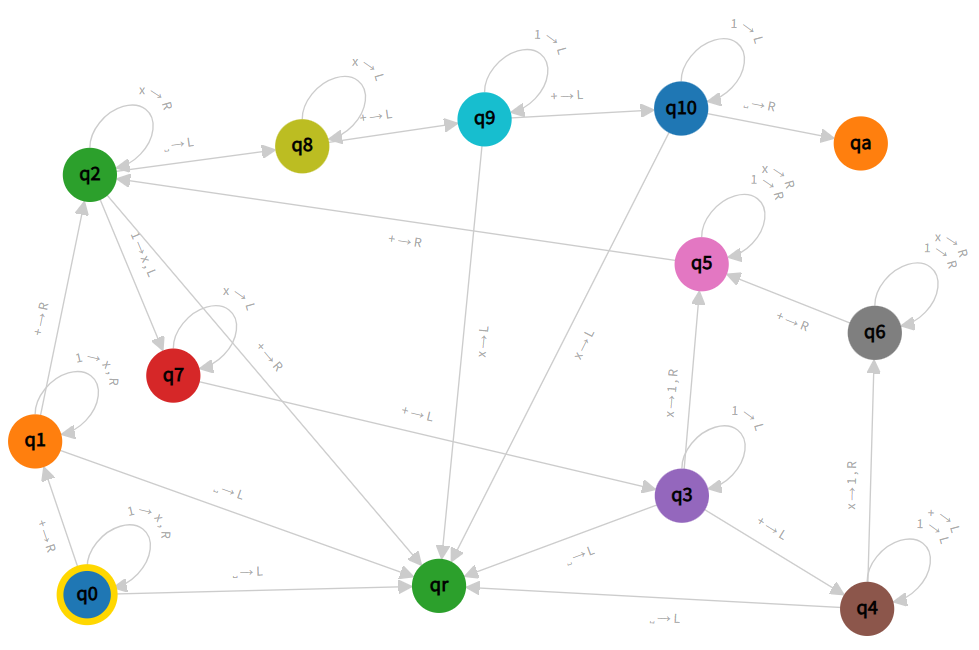
\includegraphics[scale = 0.42]{unary adder.png}

    \item \textit{Explicación de por qué la máquina es total y reconoce el lenguaje $A$}

La máquina $M$ descrita anteriormente es total, pues para cada entrada posible $w \in \Sigma^*$, $M$ acepta o rechaza. Podemos asegurar esto por la construcción de la función de transición $\delta$ esquematizada arriba, la cual impide a $M$ entrar en ciclos infinitos. En cada estado relevante hay transición para todos los símbolos de $\Gamma=\{1,\#,\times,t\}$ que pueden aparecer en la cinta; cuando se detecta una situación inválida (p. ej. falta de $\#$, tercer $\#$, etc.) la transición va a $q_r$. En los demás casos, guía el flujo a los siguientes estados de fase.

Tras la Fase 1: todos los $1$ de $\alpha$ y $\beta$ están marcados con $\times$; $\gamma$ permanece con $1$. Luego, el número de $\times$ en $\alpha\beta$ es exactamente $|\alpha|+|\beta|$. En cada iteración de las Fases 2–3/4:
  \begin{itemize}
      \item Se marca un $1$ de $\gamma$ $(1\to\times)$.
      \item Se desmarca exactamente un $\times$ de $\beta$ o, si ya no hay allí, de $\alpha$ $(\times\to 1)$.
  \end{itemize}
  Por lo tanto, el contador $n_{\times}(\gamma)$ y el contador $n_{\times}(\alpha\beta)$ restantes avanzan en sentidos opuestos y siempre al mismo ritmo (uno sube en 1 y el otro baja en 1 por iteración que continúa).

Además, si la máquina acepta es porque:
\begin{enumerate}
    \item No apareció un tercer $\#$ (formato correcto),
    \item $\gamma$ se agotó (no quedan $1$ sin marcar), y
    \item En la Fase 5 no quedó ningún $\times$ en $\alpha$ o $\beta$.
\end{enumerate}
Como invariante, el número de $1$ consumidos en $\gamma$ es igual al número de $\times$ consumidos en $\alpha\beta$. Como al aceptar ya no quedan $\times$ en $\alpha\beta$, necesariamente se consumieron todos los $|\alpha|+|\beta|$. Luego $|\gamma|=|\alpha|+|\beta|$.
  
Así, $M$ siempre se detiene y acepta exactamente las palabras de la forma $\alpha\#\beta\#\gamma$ con $|\alpha|+|\beta|=|\gamma|$. Por tanto, $M$ es total y decide el lenguaje $A$. Como $M$ decide a $A$, también $M$ reconoce a $A$.
\end{enumerate}

\item Sea $\Sigma$ un alfabeto finito. Demuestra que para todo lenguaje reconocible $A \subseteq \Sigma ^*$ existe una máquina de Turing M tal que L(M) = A y siempre que M rechaza una cadena de entrada $w \in \Sigma ^*$, lo hace entrando en un loop infinito.

  Dem.

  Sea $A \subseteq \Sigma^*$ un lenguaje reconocible cualquiera, esto quiere decir que existe una MT $N = (Q, \Sigma, \Gamma, \delta, q_0, q_{acepta}, q_{rechaza})$, tal que $L(N) = A$.

  Proponemos la siguiente máquina de Turing $M = (Q', \Sigma, \Gamma, \delta_M, q_0, q_{acepta})$ tal que

  $Q' = Q - \{q_{rechaza}\} \cup \{p\}$

  
  $\delta(q,x)_M = $
  \begin{cases}
    (p,a,L) \text{ si } \delta(q,x) = (q_{rechaza},a,L) \\
    (p,a,R) \text{ si } \delta(q,x) = (q_{rechaza},a,R) \\
    (p,x,R) \text{ si } q = p \\
    \delta(q,x)  \text{ en otro caso}
  \end{cases} para cualquier $x,a \in \Sigma$ y $q \in Q'$

  P.d $L(M)=A$

  Procedemos por doble contención
  
  P.d $A \subseteq L(M)$

  Sea $w \in A$ una cadena cualquiera, como A es reconocible, significa que w es aceptada por N. Esto implica que N llega al estado $q_{acepta}$ tras procesar esta cadena. Por la construcción de M, las transiciones de M que conducen a la aceptación son idénticas a las de N. Por lo tanto, si N acepta w, M también lo hará, así $w \in L(M)$

  P.d $L(M) \subseteq A$

  Sea $w \in L(M)$, esto quiere decir que M acepta a w. Por la construcción de M, M acepta si y sólo si N acepta, por lo tanto $w \in L(N) $ pero $L(N)=A$, así $w \in A$.

  Por lo que podemos concluir que $L(M)=A$.

  P.d Cuando M rechaza lo hace entrando a un loop infinito

  Sea w una cadena que es rechazada por N, esto sucede unicamente si la computación de w en N termina en el estado $q_{rechaza}$, ahora, según nuestra construcción de M, cualquier transición en N que hubiera llevado a $q_{rechaza}$ lleva al estado p en M. Una vez en el estado p, según la definición de $\delta_M$, no importa lo que se lea M se va a quedar en p y se va a mover a la derecha sin parar. Dado que p no es un estado de aceptación ni de rechazo, la máquina nunca se detiene. Es decir, se queda en un loop infinito.

  Así podemos concluir que para cualquier lenguaje A reconocible existe una MT M tal que $L(M)=A$ y M rechaza entrando a un loop infinito.
  
\item Sea $\Sigma$ un alfabeto finito. Demuestra que si $A \subseteq \Sigma ^*$ es un lenguaje regular, entonces A es decidible.

  

  
  \end{enumerate}
\end{document}
